\documentclass[conference]{IEEEtran}

% ==============================================PACKAGES============================================
\usepackage{listings}
\usepackage{xspace}
\usepackage[all]{xy}
\usepackage{textcomp}
\usepackage{csquotes}

\usepackage{tabularx}
\usepackage{array}
\usepackage{rotating}

\usepackage{xcolor}
\usepackage{colortbl}
\usepackage{graphicx}
\usepackage{float}

\usepackage{amsmath,amssymb,amsfonts}
\usepackage{algorithmic}
% ==================================================================================================

\def\BibTeX{{\rm B\kern-.05em{\sc i\kern-.025em b}\kern-.08em
    T\kern-.1667em\lower.7ex\hbox{E}\kern-.125emX}}
    
    
\begin{document}

% ============================================MACROS================================================
%------------------------------------------------------------------------------
%    File : ReviewMacros.tex
%  Author : Jason Jaskolka
% Version : 1.0

% This file contains macro definitions for reviewing documents.
%------------------------------------------------------------------------------
% These macros require the following package inclusions:
	% \usepackage{soul}
%------------------------------------------------------------------------------

% Color Definitions
%------------------------------------------------------------------------------
\definecolor{darkcyan}{rgb}{0.75,0.0,0.0}
\definecolor{darkgreen}{rgb}{0.0,0.6,0.0}
\definecolor{darkblue}{rgb}{0.0,0.0,0.6}
\definecolor{darkcyan}{rgb}{0.0,0.6,0.6}
\definecolor{darkmagenta}{rgb}{0.6,0.0,0.6}
\definecolor{darkamber}{rgb}{1.0,0.5,0.0}
\definecolor{darkyellow}{rgb}{0.6,0.6,0.0}
\definecolor{darkred}{rgb}{0.9,0.0,0.0}

\definecolor{lightred}{rgb}{1.0,0.9,0.9}
\definecolor{lightgreen}{rgb}{0.9,1.0,0.9}
\definecolor{lightblue}{rgb}{0.9,0.9,1.0}
\definecolor{lightcyan}{rgb}{0.8,1.0,1.0}
\definecolor{lightmagenta}{rgb}{1.0,0.8,1.0}
\definecolor{lightamber}{rgb}{1.0,0.8,0.0}
\definecolor{lightyellow}{rgb}{1.0,1.0,0.8}

\definecolor{webgreen}{rgb}{0,0.5,0}
\definecolor{webbrown}{rgb}{0.6,0,0}

\definecolor{grey}{rgb}{0.65,0.65,0.65}
\definecolor{purple}{rgb}{0.4,0,0.75}
%------------------------------------------------------------------------------

% Notes
%------------------------------------------------------------------------------
\newcommand{\mynote}[2]{
	\ifstrequal{#1}{0}{\textcolor{darkamber}{#2}}{}
  	\ifstrequal{#1}{1}{\textcolor{darkmagenta}{#2}}{}
  	\ifstrequal{#1}{2}{\textcolor{darkcyan}{#2}}{}
  	\ifstrequal{#1}{3}{\textcolor{darkgreen}{#2}}{}
  	\ifstrequal{#1}{4}{\textcolor{darkred}{#2}}{}
}
%------------------------------------------------------------------------------

% To Discuss
%------------------------------------------------------------------------------
\newcommand{\todiscuss}[2]{
	\ifstrequal{#1}{0}{\textcolor{darkamber}{\textit{\textbf{TO DISCUSS}: #2}}}{}
  	\ifstrequal{#1}{1}{\textcolor{darkmagenta}{\textit{\textbf{TO DISCUSS}: #2}}}{}
  	\ifstrequal{#1}{2}{\textcolor{darkcyan}{\textit{\textbf{TO DISCUSS}: #2}}}{}
  	\ifstrequal{#1}{3}{\textcolor{darkgreen}{\textit{\textbf{TO DISCUSS}: #2}}}{}
}
%------------------------------------------------------------------------------

% To Do
%------------------------------------------------------------------------------
\newcommand{\todo}[2]{
	\ifstrequal{#1}{0}{\textcolor{darkamber}{\textbf{\underline{TO DO}}: #2}}{}
  	\ifstrequal{#1}{1}{\textcolor{darkmagenta}{\textbf{\underline{TO DO}}: #2}}{}
  	\ifstrequal{#1}{2}{\textcolor{darkcyan}{\textbf{\underline{TO DO}}: #2}}{}
  	\ifstrequal{#1}{3}{\textcolor{darkgreen}{\textbf{\underline{TO DO}}: #2}}{}
  	\ifstrequal{#1}{4}{\textcolor{darkred}{\textbf{\underline{TO DO}}: #2}}{}
}
%------------------------------------------------------------------------------

% To Address
%------------------------------------------------------------------------------
\newcommand{\toaddress}[2]{
	\ifstrequal{#1}{0}{~\\\noindent\textcolor{darkamber}{$\bigstar$~\textbf{#2}}\\}{}
  	\ifstrequal{#1}{1}{~\\\noindent\textcolor{darkmagenta}{$\bigstar$~\textbf{#2}}\\}{}
  	\ifstrequal{#1}{2}{~\\\noindent\textcolor{darkcyan}{$\bigstar$~\textbf{#2}}\\}{}
  	\ifstrequal{#1}{3}{~\\\noindent\textcolor{darkgreen}{$\bigstar$~\textbf{#2}}\\}{}
}
%------------------------------------------------------------------------------

% To Revise
%------------------------------------------------------------------------------
\newcommand{\torevise}[1]{
    {\textcolor{darkred}{\textbf{\underline{TO REVISE}}: #1}}{}
}

% Track Changes
%------------------------------------------------------------------------------
\newcommand{\add}[1]{\textcolor{darkgreen}{#1}}
\newcommand{\remove}[1]{\textcolor{red}{\st{#1}}}
\newcommand{\replace}[2]{\remove{#1}~\add{#2}}
\newcommand{\suggest}[1]{\noindent\textcolor{blue}{$\circ$---~\textit{#1}~---$\circ$}\\}
%------------------------------------------------------------------------------
% ===================================STATE VARIABLES=====================================
\newcommand{\var}[1]{\texttt{#1}\@\xspace}              % for state variables
\newcommand{\val}[1]{\texttt{#1}\@\xspace}              % for state variable values
\newcommand{\func}[1]{\texttt{#1}\@\xspace}             % for functions
\newcommand{\sync}[1]{\texttt{#1}\@\xspace}             % for synchronizations messages
\newcommand{\notation}[1]{\emph{#1}\@\xspace}           % for explaining UPPAAL notations
\newcommand{\state}[1]{\texttt{#1}\@\xspace}            % for states/locations

% Symbols only (S = symbol)
\newcommand{\CNC}{\textrm{CNC}\@\xspace}
\newcommand{\RPT}{\textrm{RPT}\@\xspace}
\newcommand{\LDR}{\textrm{LDR}\@\xspace}
\newcommand{\DA}{\textrm{DEV\_A}\@\xspace}
\newcommand{\DB}{\textrm{DEV\_B}\@\xspace}
\newcommand{\AC}{\emph{Always-Connected}\@\xspace}
\newcommand{\RC}{\emph{Reboot-Capable}\@\xspace}
% ==================================================================================================




% =============================================TITLE================================================
\title{Analyzing the Impact of Rebooting and Network Degradation on IoT Botnets using Timed Automata}
% ==================================================================================================


% ============================================AUTHORS===============================================
\author{\IEEEauthorblockN{Alvi Jawad, Luke Newton\\}
    \IEEEauthorblockA{Systems and Computer Engineering Department \\
    Carleton University, Ottawa, Ontario \\
    \{alvi.jawad, luke.newton\}@carleton.ca \\
    }
}
% ==================================================================================================



\maketitle



% ============================================Abstract==============================================
\begin{abstract}
\fontsize{10pt}{12pt}\selectfont
\label{abstract}
% Begin Section
The Internet of Things (IoT) has stimulated the creation of a new era with the promise of ubiquitous connectivity aided by a proliferation of inexpensive IoT devices. The threat presented by the recent rise of botnets and their capability to infect numerous vulnerable IoT devices on the internet mandate a better understanding of their inner workings and investigation of alternative defensive mechanisms usable by \textbf{resource-constrained IoT devices}. In this project, we aim to model and simulate the dynamic behavior of the Mirai botnet as a network of timed automata using the modeling tool UPPAAL to delve deeper into the botnet infection process. Additionally, to determine its feasibility as a defensive measure, we examine the effectiveness of rebooting and network degradation on varying system configurations. The resulting formal analysis provides a solid understanding of the impact of such mechanisms on botnet growth and insight into their efficacy to weigh them against other available countermeasures.


% \torevise{The Internet of Things (IoT) has stimulated the creation of a new era with the promise of ubiquitous connectivity. Recent years have seen a proliferation of cheap IoT devices, many of which employ energy-efficient designs, mandating low computational resources that preclude the use of rigorous security mechanisms. Furthermore, many deployed IoT devices continue to use default vendor passwords, and many others tend to have weak credentials. Adversaries in IoT exploit these security vulnerabilities to create their own army of connected IoT devices, known as botnets, only to be used later to perform various malicious attacks on the network. In this project, we aim to model and simulate the dynamic behavior of a botnet as a networked timed automata using the modeling tool UPPAAL to gain insight into the botnet infection process in diverse system configurations. Additionally, we aim to analyze the impact of the infection process on the modeled network by implementing existing security mechanisms and assess the feasibility of such measures.}

% The threat presented by the recent rise of botnets and their capability to infect numerous vulnerable IoT devices on the internet mandates a better understanding of their inner workings and investigation of alternative defensive mechanisms usable by resource-constrained IoT devices. 

% The knowledge gained through this study allowed us to reinforce our understanding of the botnet infection process as well as identify areas of limited understanding such as suggested frequency and duration of device rebooting. Additionally, they will gain insight into the effectiveness and viability of rebooting and weigh it against other available defensive measures to provide suitable recommendations.


% End Section
\end{abstract}
% ==================================================================================================


% ============================================KEYWORDS==============================================
\begin{IEEEkeywords}
\fontsize{10pt}{12pt}\selectfont
Internet of Things (IoT), Botnets, Network Security, Modeling and Simulation, Timed Automata, Impact Analysis, Rebooting, UPPAAL
\end{IEEEkeywords}
% ==================================================================================================





% ============================================CONTENTS==============================================
\section{Introduction}
\fontsize{10pt}{12pt}\selectfont
\label{sec:introduction}
% Begin Section
 
The Internet of Things (IoT) refers to the interconnected network of the vast number of internet-enabled physical objects around the world. In recent years, the increased availability of low cost, low power sensors, and enhanced communication methods has caused an explosion in the number of IoT devices~\cite{atzori2010_IoT_Survey}. With this increased communication, data collection, and analysis, IoT has the potential to improve many facets of society, including, but not limited to, healthcare, infrastructure, supply chains, and the general home and office environments. Unfortunately, due to the relatively low computational resources available for typical IoT devices and the rushed production of many such devices, the IoT infrastructure has become vulnerable to a number of security threats~\cite{alaba2017_IoT_Security_Survey}.

Botnets are one of the major security issues faced in the current IoT landscape~\cite{silva2013_Botnet_Survey}. Botnets are a network of devices corrupted by malware that are ready to be instructed by a bot-master through some Command and Control infrastructure. Once in control of a large enough botnet, botmasters may either use or trade the attacking capabilities in exchange for money to perform targeted attacks on websites~\cite{kolias2017_Mirai_DDoS}. The relatively low computational resources of cheap IoT devices imply the lack of built-in measures to protect against malware~\cite{bertino2017_Botnets_IoT}. Furthermore, IoT devices are often deployed with weak and/or default credentials, and the embedded nature of the devices can make it challenging, and often impossible, to patch vulnerabilities. All this comes together to make IoT devices ideal candidates for botnet infection.

While bots in an IoT botnet do not individually present a threat, a large enough botnet can cause catastrophic impacts. One such example is the Mirai botnet, first identified in 2016, that launched Distributed Denial of Service (DDoS) attacks against security blog KrebsOnSecurity and French cloud computing company OVH, with malicious traffic peaking at 620 Gbps and 1.1 Tbps respectively~\cite{kolias2017_Mirai_DDoS}. More recently, the largest ever DDoS attack was targeted at Amazon Web Services in February 2020, which saw sustained traffic at 2.3 Tbps~\cite{cloudflare_DDoS}. While the majority of the botnet exploits involve DDoS attacks, they are not limited to DDoS attacks only. The following lists several malicious capabilities of botnets:
\begin{enumerate}
    \item DDoS: The most common botnet attack. A large enough botnet can flood network endpoints or links with enough traffic to severely degrade or completely disallow legitimate traffic through the targeted location~\cite{silva2013_Botnet_Survey}.
    \item General bot traffic: Continuous communication and propagation consumes network bandwidth and often results in decreased performance in infected devices.
    \item Spam or Malware dissemination: Rather than sending all bot traffic to one location like in a DDoS attack, botnets can also be used to distribute malicious payloads to a wide variety of targets~\cite{silva2013_Botnet_Survey}.
    \item Firmware corruption: Botnets like BrickerBot can, once commanded, access and destroy a device's firmware~\cite{kolias2017_Mirai_DDoS}.
\end{enumerate}
Research on botnets has surged in popularity after the emergence of the Mirai Botnet, and our research intends to build on top of these efforts.

The rest of this proposal is structured as follows. Section~\ref{sec:problem_statement} explores the motivation behind our study and presents our research objectives. Section~\ref{sec:work_plan} outlines how we plan to approach our proposed modeling and analysis through various stages of the project. Finally, Section~\ref{sec:expected_final_outcome} describes our envisioned expected outcomes from the project.

% End Section

\section{Background}
\fontsize{10pt}{12pt}\selectfont
\label{sec:background}
% Begin Section
In this section, we introduce the timed automata modeling formalism, the UPPAAL modeling tool, and some relevant terminologies and concepts used throughout this paper.

% ===================================== Timed Automata ======================================
\subsection{Timed Automata}
\label{sub: timed_automata}
Timed automata is a hybrid mathematical modeling formalism in which a finite set of real-valued clocks are used to represent continuous time in a discrete-event system~\cite{alur1994_Theory_Timed_Automata}. Any real-time system whose behavior involves a predetermined set of actions can be represented as a network of timed automata. The system can be decomposed into its constituent components, and each component can be modeled as a timed automaton, which is a finite-state machine extended with clock variables~\cite{behrmann2004_Tutorial_UPPAAL}. A timed automaton is a tuple $(L, lo, C, A, E, I)$ where,
\par
$L$ is a set of locations
\par
$lo \in L$ is the initial location
\par
$C$ is the set of clocks 
\par
$A$ is a set of actions, co-actions, and the internal $\tau$-action
\par
$E \subseteq L \times A \times B(C) \times 2c \times L$ is a set of edges
\par
$I : L \to B(C)$ assigns invariants to locations 
\par
A timed automaton accepts timed words; infinite sequences in which each symbol is associated with a real-valued time of occurrence~\cite{alur1994_Theory_Timed_Automata}. At the simulation start, every single automaton in a network of timed automata begins with all of its clocks initialized to zero. The elapsed time is reflected in the change of clocks, representing the advance of time in reality. All clocks are independent of each other and can be reset at each transition to keep track of the elapsed time since the last reset. A transition may only be taken if the associated time constraint imposed upon that transition is satisfied by the current clock values. This feature allows us to model the timing properties of real-time systems and capture interesting qualitative and quantitative aspects such as periodicity, bounded response, and timing delays.

% ========================================== UPPAAL ===========================================
\subsection{Modeling in UPPAAL}
\label{sub: modeling_in_uppaal}
UPPAAL is an integrated tool environment that supports the modeling, validation, and verification of real-time systems as networks of timed automata~\cite{behrmann2004_Tutorial_UPPAAL}. The model can be extended with data types (e.g., bounded integers, arrays) while also allowing model checking for verification and validation of system properties. This academic endeavor, jointly developed by Uppsala University in Sweden and Aalborg University in Denmark, has received considerable research community support for research on timed automata in recent years. Our work uses the UPPAAL 4.1 development snapshot available under a free academic license\footnote{http://www.uppaal.org/}.
\par
% UPPAAL basic graphical notations figure
\begin{figure}[h!]
    \centering
    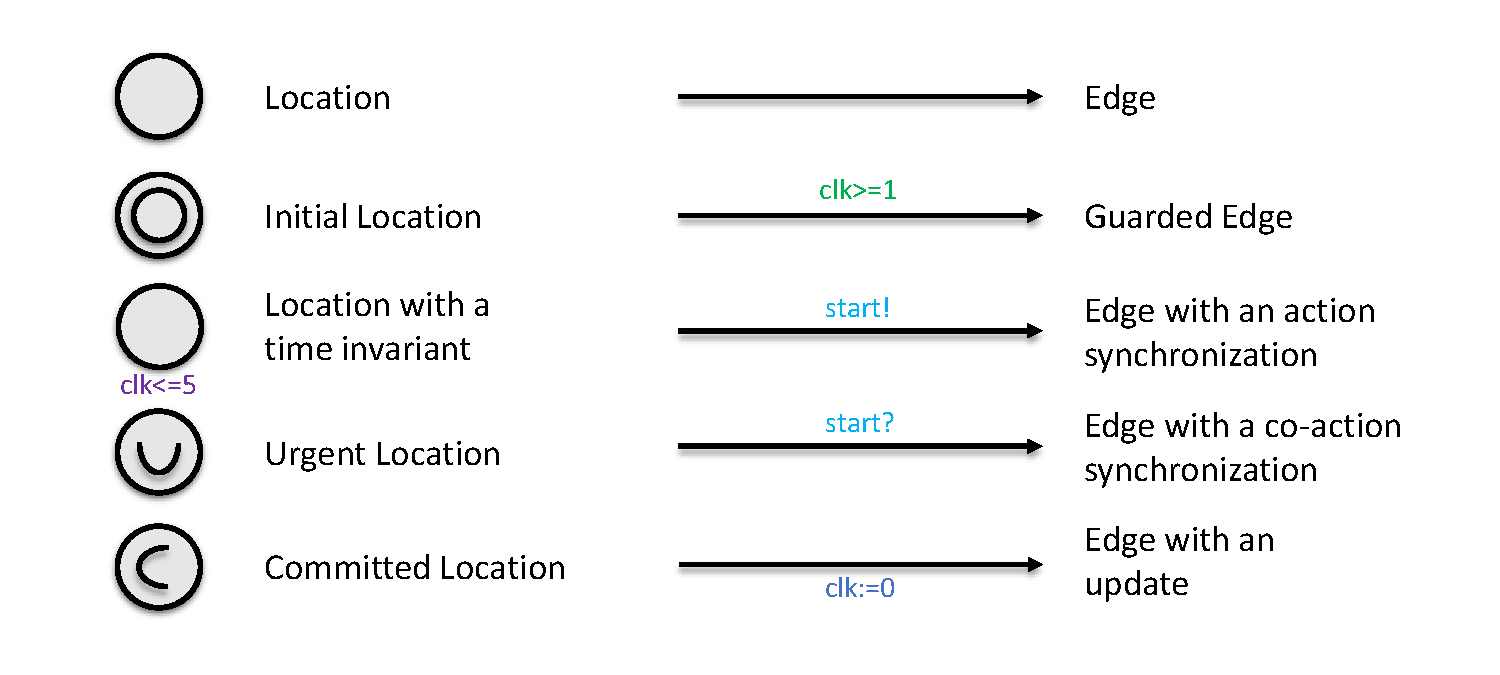
\includegraphics[width=\linewidth]{Figures/UPPAAL_Notations.pdf}
    \caption{UPPAAL graphical notations}
    \label{fig:uppaal_graphical_notations}
\end{figure}
\par
Figure~\ref{fig:uppaal_graphical_notations} shows some basic graphical notations used to model real-time systems in UPPAAL. Circles denote regular \notation{locations} that represent the state of an automaton performing a specific function. The \notation{initial location} (only one) of every automaton is depicted by an additional inner circle, specifying the starting behavior of that automaton when the system starts. Regular and \notation{initial locations} can be accompanied by a time invariant (depicted in violet text), which are time constraints imposed upon the location. A location with a time invariant must be left within the specified time constraint. Locations are also called \notation{states}, which is the term we will be using extensively throughout the paper.
\par
\notation{Urgent states}, denoted by an additional U inside the circle, represent states that are time-critical. These states cannot have any time invariants, and no time can pass while an automaton is in such a state. However, if any other automaton in the network is capable of performing an instantaneous action, that action is allowed. \notation{Committed states} (marked by an additional C) are even more restricted states that allow neither the passage of time nor any action by any other automaton unless that state is left.
\par
\notation{Edges}, depicted by arrows, represent the transition from one state to another. UPPAAL uses a handshaking mechanism to synchronize communication between different automata. During a transition, an \notation{edge} can send an action synchronization message (depicted in light blue text). This action message (\sync{start!}) must synchronize with another \notation{edge} with a corresponding co-action synchronization message (\sync{start?}), enabling the latter transition to take place.
\par
Individual automata can use state variables to record and share their state with other automata in the network. In addition, clock variables can be used to record the passage of time and impose timing constraints on locations and transitions. \notation{Guarded Edges} represent guarded transitions, where the transition is only allowed once the conditions (depicted in green text) imposed using state and/or clock variables on the transition, are satisfied. Additionally, edges can be accompanied by an \notation{update} command (depicted in blue text) that updates the value of a state and/or clock variable once the transition is completed.
\par
% End Section

\section{Botnets in IoT}
\fontsize{10pt}{12pt}\selectfont
\label{sec:botnets}
% Begin Section
% ======================================== What are botnets? =========================================
Botnets are one of the major security issues faced in the current IoT landscape~\cite{silva2013_Botnet_Survey}. Recent years have seen considerable growth in both original and different variants of botnets, causing a significant impact on various aspects of IoT networks~\cite{kolias2017_Mirai_DDoS}. This section summarizes the impact of recent botnet attacks and explores the threat landscape of modern IoT networks.
\par

% Start Subsection***********************************************************************************
\subsection{The Impact of Botnets}
\label{sub:impact_of_botnets}
% ====================================== Recent botnet attacks =======================================
A botnet is a network of devices compromised by malware that can be instructed by a botmaster through a Command and Control (C\&C) infrastructure. Although individual bots in an IoT botnet do not pose a threat, a large enough botnet can have catastrophic impacts. One prime example of this is the Mirai botnet, which launched Distributed Denial of Service (DDoS) attacks against security blog KrebsOnSecurity and French cloud computing company OVH, with malicious traffic peaking at 620 Gbps and 1.1 Tbps respectively in 2016~\cite{kolias2017_Mirai_DDoS}. More recently, the largest ever DDoS attack was targeted at Amazon Web Services in February 2020, which saw sustained traffic at 2.3 Tbps~\cite{cloudflare_DDoS}.
\par
Contrary to the majority of exploits involving DDoS attacks, botnets are not limited to DDoS attacks alone. The following lists several malicious capabilities of botnets~\cite{kolias2017_Mirai_DDoS, silva2013_Botnet_Survey}:
\begin{enumerate}
    \item DDoS: A large enough botnet can flood network endpoints or links with enough traffic to severely degrade or completely disallow legitimate traffic through the targeted location.
    \item General bot traffic: Continuous communication and propagation consumes network bandwidth and can result in decreased performance in infected devices.
    \item Spam or Malware dissemination: Rather than sending all bot traffic to one location like in a DDoS attack, botnets can also be used to distribute malicious payloads to a wide variety of targets.
    \item Firmware corruption: Botnets like BrickerBot, once commanded, can access and destroy a device's firmware.
\end{enumerate}
% End Subsection**************************************************************************************


% Start Subsection***********************************************************************************
\subsection{The Threat to IoT}
\label{sub:threat_to_iot}
% =========================== Why should we care? (threats to our network) ===========================

% old version:
%IoT, with its sheer number of vulnerable connected devices, has become a tempting target for botmasters. At its peak, Mirai may have held up to 400,000 connected devices, hinting at a small picture of what could happen if all of these infected devices were used simultaneously to perform an attack~\cite{kolias2017_Mirai_DDoS}. The relatively low computational resources of inexpensive IoT devices imply the lack of built-in measures to protect against malware~\cite{bertino2017_Botnets_IoT}. Off-the-shelf IoT devices are rarely designed with security in mind, and the use of lightweight operating systems and network protocols means that the device and its communications are inherently vulnerable to various attacks. Moreover, a large proportion of IoT devices are deployed with their initial configuration and easily guessable weak and/or default credentials, and the embedded nature of these devices can make it challenging, often impossible, to patch vulnerabilities. All of these come together to make IoT devices ideal candidates for botnet infection and present a greater need to explore alternatives to the defenses conventional computers would typically employ.

IoT, with its sheer number of vulnerable connected devices, has become a tempting target for botmasters. At its peak, Mirai may have held up to 400,000 connected devices, hinting at a small picture of what could happen if all of these infected devices were used simultaneously to perform an attack~\cite{kolias2017_Mirai_DDoS}. Off-the-shelf IoT devices are rarely designed with security in mind, and their relatively low computational resources mean that defenses used by more conventional computers, such as anti-malware software, are not feasible to implement. Moreover, a large proportion of IoT devices are deployed with their initial configuration and easily guessable weak and/or default credentials, and the embedded nature of these devices can make it challenging, often impossible, to patch vulnerabilities. All of these come together to make IoT devices ideal candidates for botnet infection and present a greater need for research into botnet behaviors and the evaluation of possible defenses.
\par
% ============================= Why are we looking at rebooting? =============================
Rebooting has been suggested as an effective defensive mechanism to control the spread of botnets~\cite{tanaka2019_PN_Botnet}. While botnets can be used by the botmasters for their sole gain, they can also lend the attacking capabilities of a large-enough botnet to external interested parties in exchange for something valuable~\cite{kolias2017_Mirai_DDoS}. The precondition behind this contract is the possession of a large attack-capable botnet and the maintainability of the botnet size over an extended period. One core theme of our analysis of the botnet infection process is to see whether rebooting alone is capable of preventing the attacker from amassing and/or maintaining their attacking capability over a certain period. If so, we wish to see what rate of rebooting is the most effective and whether such a frequency is feasible for an actual IoT device.
% End Subsection**************************************************************************************

% End Section

\section{Modeling the Infection Process}
\fontsize{10pt}{12pt}\selectfont
\label{sec:modeling}
% Begin Section
To model the botnet under study, Mirai, with the final objective of performing our feasibility analysis, we first need to understand the Mirai infection process, all the entities involved in the process, and how these entities interact with each other. In this section, we detail the Mirai infection process and present our timed automata model of the Mirai botnet developed in UPPAAL.
% Mirai Infection Process
\begin{figure}[h!]
    \centering
    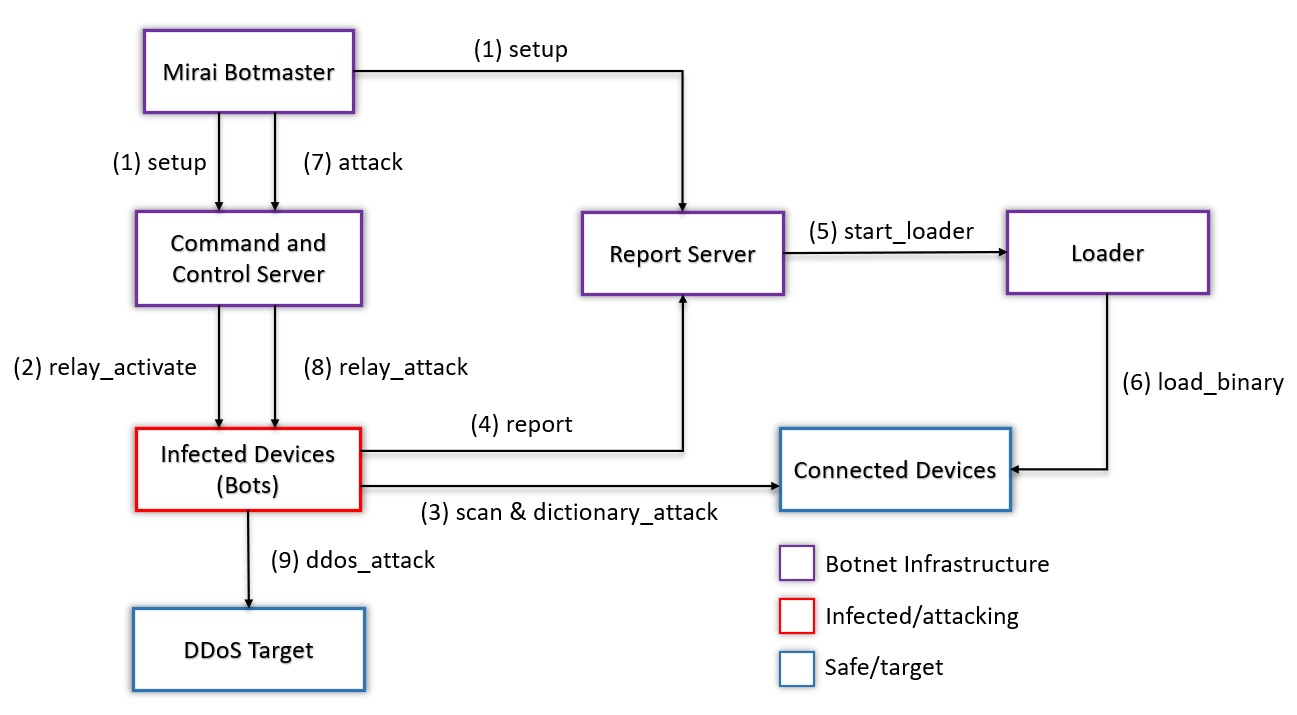
\includegraphics[width=\linewidth]{Figures/mirai_infection_process.jpg}
    \caption{Mirai Infection Process}
    \vspace{-0.2 cm}
    \label{fig:mirai_infection_process}
\end{figure}
\par


% Start Subsection**************************************************************************************
\subsection{Mirai Infection Process}
\label{sub:mirai_infection_process}
% ====================================== The entities involved =========================================
Mirai falls under the category of classical centralized botnets that revolve around a single central C\&C server to spread~\cite{shanmughapriya2018_botnet_of_things_survey}. Figure~\ref{fig:mirai_infection_process} illustrates the primary components of the centralized infrastructure (a C\&C server, a Report server, and a Loader) as well as the way these components interact. These entities are under the control of the Mirai botmaster, who actuates and directs the botnet activity through the infrastructure. The botnet is also comprised of the devices that have already been infected, also known as bots, that actively seek out other vulnerable connected devices in the network to infect. The bots under control can be further directed to compromise a DDoS target with a variety of DDoS attacks under Mirai's disposal~\cite{kambourakis2017mirai}.
\par
% ==================================== Steps: Mirai Infection Process ====================================
The Mirai infection process can be outlined in a number of simplified steps~\cite{kambourakis2017mirai, Antonakakis2017_USENIX_Mirai_First_Study}:
\begin{enumerate}
    \item The botmaster begins the infection process by setting up the remote C\&C server and the Report server.
    \item The C\&C server activates the first bot, one that is infected from the beginning, to initiate the scan-attack-report cycle of a bot.
    \item The bot statelessly scans the network for open Telnet ports at randomly selected IP addresses, and initiates a brute force remote-login attempt by randomly selecting 10 out of the 62 default or commonly used credentials hard-coded in the Mirai binary.
    \item If a brute force attack is successful, the attacking bot reports the victim \emph{id} (device IP and the credentials that worked) to the Report server.
    \item If the reported device is not part of the botnet, the report server adds it to its records, and subsequently, activates the Loader to load the malware binary into the new vulnerable device.
    \item The Loader determines the architecture of the target device and uploads a hardware-specific malware, transforming the target device into another bot. Steps 3 to 6 continue until the botnet is large enough for the attacker's purpose or about all the vulnerable devices in the network have been compromised.
    \item Any time, ideally with an adequately sized botnet, the botmaster can issue an attack command to the C\&C server.
    \item The C\&C server relays the attack command to all the bots that are currently under control.
    \item The bots stop their usual scan-attack-report cycle and start performing a DDoS and/or other malicious attacks on the attack target.
\end{enumerate}
% End Subsection******************************************************************************************



% Start Subsection****************************************************************************************
% ================================== Modeling the Botnet Infrastructure ==================================
\subsection{Modeling the Mirai Botnet Infrastructure}
\label{sub:modeling_botnet_infrastructure}
We start by modeling the key entities - the C\&C server, the Report server, and the Loader - in the Mirai botnet infrastructure. Each entity is modeled as a separate automaton that engages in multiple channel synchronizations to reflect the behavior of a botnet in a real-time network. For a brief discussion about the notations used extensively throughout the modeling process, please refer to section~\ref{sub: modeling_in_uppaal}.
% The CnC server automaton
\begin{figure}[H]
    \centering
    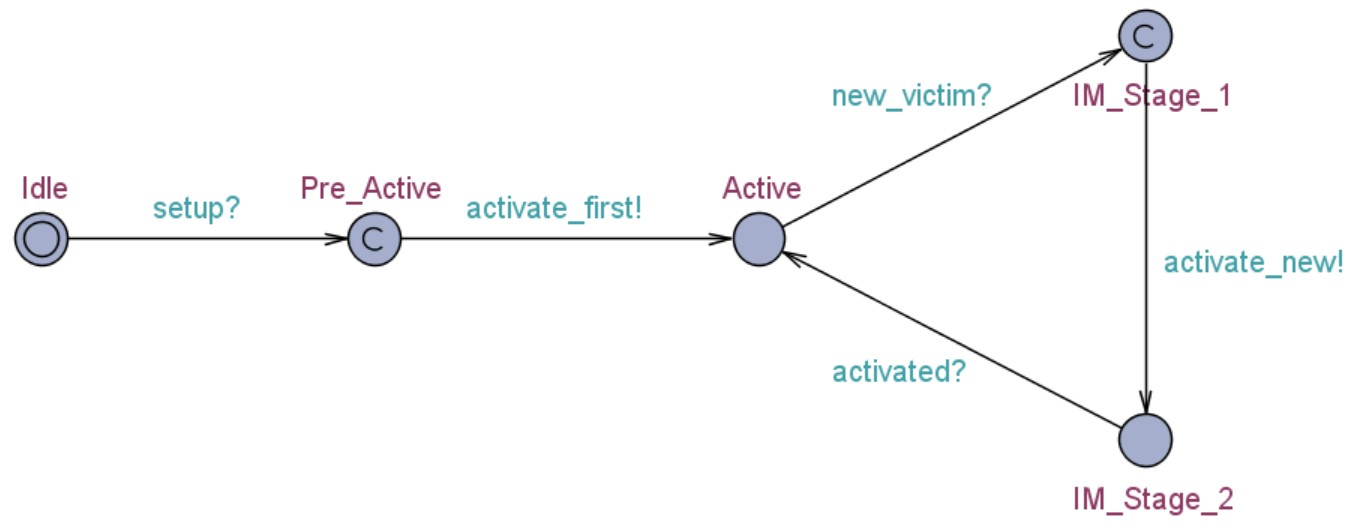
\includegraphics[width=\linewidth]{Figures/CnC_srv_automaton.jpg}
    \caption{The Command and Control Server Automaton (\CNC)}
    \vspace{-0.3 cm}
    \label{fig:CnC_server_automaton}
\end{figure}
\par
Figure~\ref{fig:CnC_server_automaton} presents the Command and Control server automaton (\CNC) with its two primary states \state{Idle} and \state{Active}. The server is set up by the abstract Mirai botmaster entity, after which \CNC activates the first bot (pre-infected) and transitions to its \state{Active} state. In this state, \CNC waits for raw socket connections from new victims, only to activate them later so they can start their own infection process.
% The Report server automaton
\begin{figure}[h!]
    \centering
    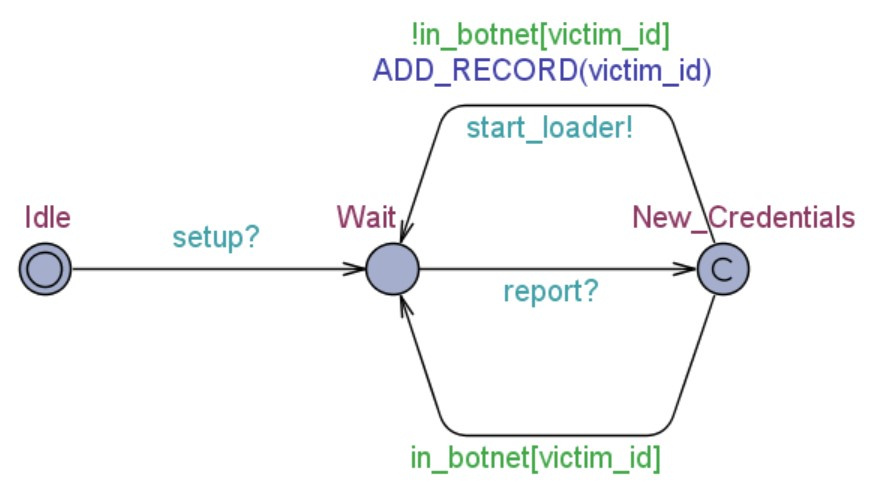
\includegraphics[width=.65\linewidth]{Figures/Report_srv_automaton.jpg}
    \caption{The Report Server Automaton (\RPT)}
    \vspace{-0.1 cm}
    \label{fig:report_server_automaton}
\end{figure}
\par
Figure~\ref{fig:report_server_automaton} illustrates the behavior of the Report server automaton (\RPT). Similar to \CNC, \RPT is also set up the Mirai botmaster, allowing the transition from the \state{Idle} state to the \state{Wait} state. Once in the \state{Wait} state, the \RPT listens for incoming reports of a new victim \emph{id} sent via each bot on port 80 every minute. Any new \emph{id} is checked against the current records. \LDR adds a new record as well as activates the Loader automaton if the \emph{id} proves to be a vulnerable device that is yet to be infected.
% The Loader automaton
\begin{figure}[h!]
    \centering
    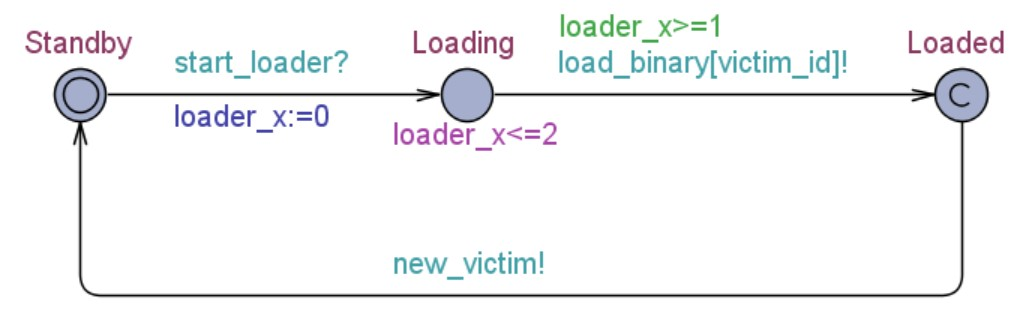
\includegraphics[width=.8\linewidth]{Figures/Loader_automaton.jpg}
    \caption{The Loader Automaton (\LDR)}
    \vspace{-0.1 cm}
    \label{fig:loader_automaton}
\end{figure}
\par
% The image is here only for formatting purposes
% Device type 1 - Always Connected
\begin{figure*}[t!]
    \centering
    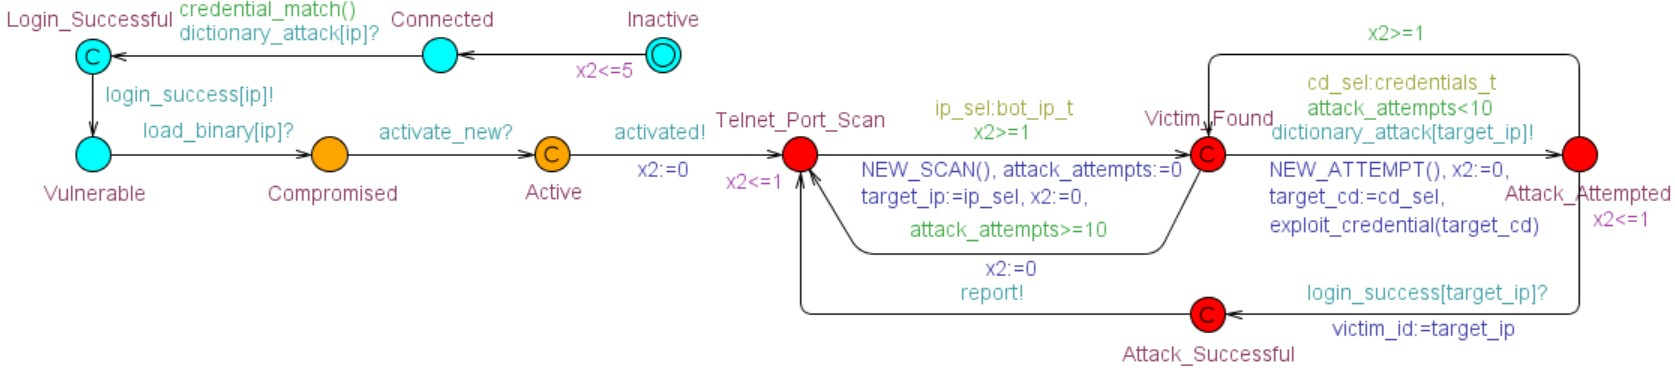
\includegraphics[width=\linewidth]{Figures/Device_t1_automaton.jpg}
    \caption{Device Automaton A (\DA) - Always-Connected}
    \vspace{-0.1 cm}
    \label{fig:device_type_a}
\end{figure*}
\par
Figure~\ref{fig:loader_automaton} shows the Loader automaton (\LDR) that reflects the inner workings of the proxies called loaders~\cite{kambourakis2017mirai}. \LDR moves from its initial \state{Standby} state to the \state{Loading} state after it has received the start\_loader command from the report server along with a vulnerable victim \emph{id}. In the \state{Loading} state, \LDR takes anywhere between one to two time units to log into the victim using the provided \emph{id} and instructs the victim to download and execute the hardware-appropriate binary, essentially turning the victim into a functional bot. After this process is over, \LDR informs \CNC about this new botnet member and returns to its \state{Standby} state.
% End Subsection******************************************************************************************



% Start Subsection****************************************************************************************
\subsection{Modeling Always-Connected Devices}
\label{sub:modeling_always_connected_devices}
After the botnet infrastructure, we focus our attention on modeling the individual device behavior inside the botnet. The device behavior here refers to the behavior when the device acts as a normal device as well as when the device is infected and being used by the botmaster for their nefarious purposes. Figure~\ref{fig:device_type_a} shows our first device automaton (\DA) where the states involved in the three different modes of behavior - (1) when the device behaves like a regular device,  (2) when it is being infected, as well as (3) when it is acting as a bot - are marked in colors blue, orange, and red, respectively.
\par
% =========================================== The device mode =============================================
\AC devices, according to RFC 7228, are representative of IoT devices that are always-on (P9) and stay connected to the network all the time~\cite{RFC_7228}. All the states marked in blue represent the regular and intended behavior of a device. \DA starts in the \state{Inactive} state and connects to the network after a specific time (within five time units of the simulation start in our model), moving to its \state{connected} state. This is the only state where another \DA in their infected mode (red) can perform dictionary attacks on a \DA. If an attack is performed with a matching credential, then \DA moves to its \state{vulnerable} state where it now has its \emph{id} leaked to the report server.
\par
% ==================================== The transition into a bot phase ====================================
States depicted in Orange represent the transition state of a device during its infection process. In the \state{Vulnerable} state, the device can be logged in to download the Mirai binary into the device. Once this process is complete, \DA moves to the compromised state, where it waits to establish a raw socket connection with the C\&C server to receive further commands. After establishing the connection, \DA moves to the \state{Telnet\_Port\_Scan} state where it now starts to act upon the commands relayed by the C\&C server.
% ========================================= The infected mode: bot ========================================
The red states in the right portion of \DA represent the same device's behavior once it is infected, activated, and has started performing activities befitting that of a bot. In the \state{Telnet\_Port\_Scan} state, the infected device now statelessly scans the network for pseudorandom IPv4 addresses for open Telnet 23 ports, and once found, moves to the \state{Victim\_Found} state. This is the state where a bot tries to gain a working Linux shell, attempting to randomly select and use 10 out of 62 hardcoded default or commonly used credentials stored in the original Mirai binary~\cite{kambourakis2017mirai}. An unsuccessful attack chain of ten takes the bot back to the \state{Telnet\_Port\_Scan} state, whereas a successful attack leads to the \state{Attack\_Successful} state first, where the victim information is reported to the Report server.
\par
% ====================================== IF space: talk about timing ======================================
% End Subsection******************************************************************************************


% Start Subsection****************************************************************************************
\subsection{Modeling Reboot-Capable Devices}
\label{sub:modeling_reboot_capable_devices}
Next, we model the behavior of devices that are capable of rebooting and reconnecting to the network once rebooted. This capability is crucial as the Mirai binary is stored in the dynamic memory and is cleared once an infected device is rebooted, essentially restoring the regular device behavior~\cite{tanaka2019_PN_Botnet}. To introduce rebooting to our device automaton, we present a modified automaton in figure~\ref{fig:device_type_b} with this capability.
\par
% The image is here only for formatting purposes
% Device type 2 - Reboot Capable
\begin{figure*}[t!]
    \centering
    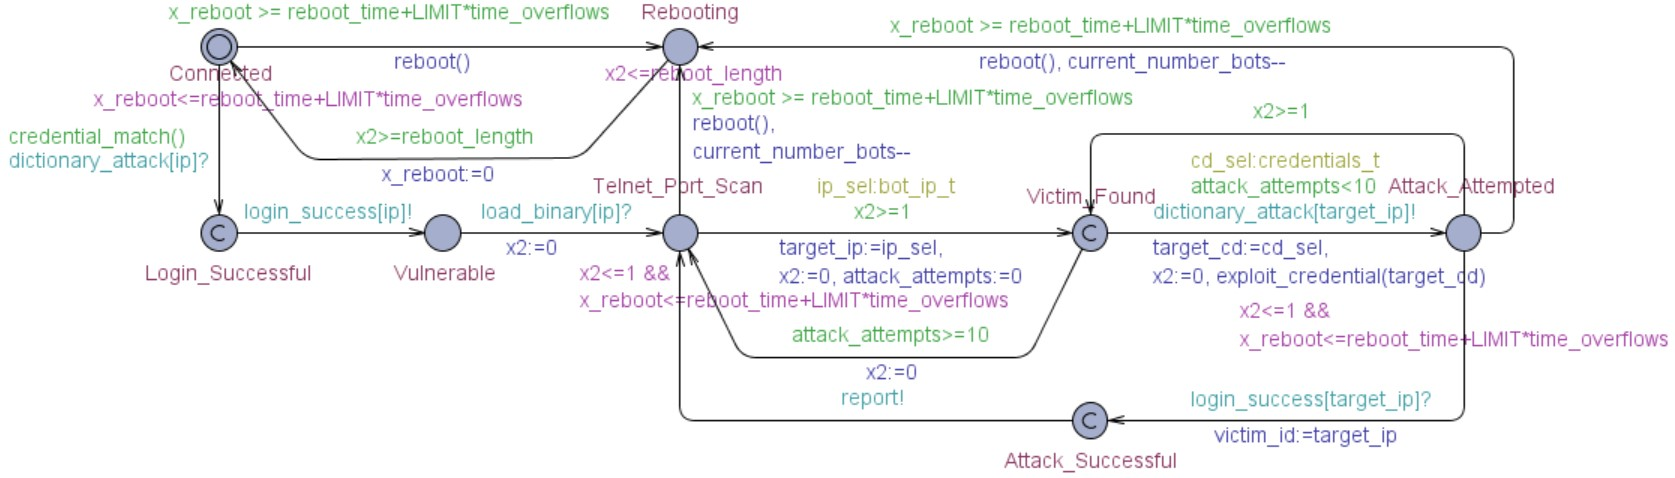
\includegraphics[width=\linewidth]{Figures/Device_t2_automaton.jpg}
    \caption{Device Automaton B (\DB) - Reboot-Capable}
    \label{fig:device_type_b}
    \vspace{-0.3 cm}
\end{figure*}
\par

% ======================================= Device Clusters: Reboot =========================================
Our second device automaton (\DB) represents clusters of \RC devices that can reboot either periodically or manually with user intervention. One particular example of this would be router configurations that allow a router to preserve its health by turning off for an hour each day when not under use. Devices of category E1 (battery-powered devices with a fixed primary battery replacement interval) and P0 (normally turned off, only attached to the network when needed), also fall under the same category and can be modeled with simple attunement of the timing constraints~\cite{RFC_7228}.
\par
% ======================================== The Reboot Capability ==========================================
\DB is extended with two new adjustable parameters for rebooting. Each device of type \DB now starts with a \emph{reboot\_time} that represents a predetermined time after which each device will turn off, moving to the \state{Rebooting} state regardless of its infection status. Additionally, another parameter, \emph{reboot\_length}, determines how much time a device takes to reboot and/or the time a device stays off after turning off. These parameters can be adjusted all at once or manually before each simulation, and the fact that we can represent stochastic timing behavior gives us great flexibility in modeling the various device clusters mentioned before. Moreover, this lets us model different distributions of various devices of type \DB, or \DA and \DB combined, and allows us to extend the model with other device automatons (e.g., with patching capability) in the future.
% End Subsection******************************************************************************************
% End Section

\section{Experimental Results}
\fontsize{10pt}{12pt}\selectfont
\label{sec:experimental_results}
% Begin Section
Finally, we perform simulations to verify the correctness of the model as well as to simulate an IoT network with varying network configurations. In this section, we present the experimental results of our simulation runs using the model developed in the previous section.

% ===================================== Simulation Parameters ======================================
\subsection{Device Type Comparison}
\label{sub:device_type_comparison}
In all simulations, all devices connected to the network are considered to be using a weak and/or default password, and as such, are vulnerable to a Mirai infection. All infected devices will use a malware binary with a dictionary consisting of 62 commonly used credentials to attack. Unless otherwise mentioned, all devices are one of two types: \AC or \RC, as described in sections~\ref{sub:modeling_always_connected_devices} and~\ref{sub:modeling_reboot_capable_devices}.
\renewcommand{\arraystretch}{1.5}
\begin{table}[h]
    \caption{\label{table:parameters}System Parameters}
    \begin{tabularx}{\linewidth}{| m{0.35\linewidth} c c |}
       \hline 
    	\multicolumn{1}{|c}{Parameter} & Default Value & Other Values Used\\
    	\hline 
    	Number of devices & 100 & 250, 500\\ 
    	Round Trip Time & 100ms & 1s\\ 
    	Simulation time & 1 day & 1 week\\ 
    	Reboot frequency  & 24hr & 1hr, 30min, 10min, 5min\\ 
    	Percentage of time bots propagate malware & 100\% & 50\%, 10\%, 1\%\\ 
    	\hline
    \end{tabularx}
\end{table}
\renewcommand{\arraystretch}{1}
\par
In addition to these constant parameters, Table~\ref{table:parameters} summarizes the adjustable parameters in our model. We perform multiple sensitivity analyses by capturing the model behavior with all parameters set to default and then adjusting one parameter at a time to observe variations in behavior. This allows us to examine how different attributes of the malware, or that of the device network, impact botnet growth. 

\begin{figure}[H]
    \centering
    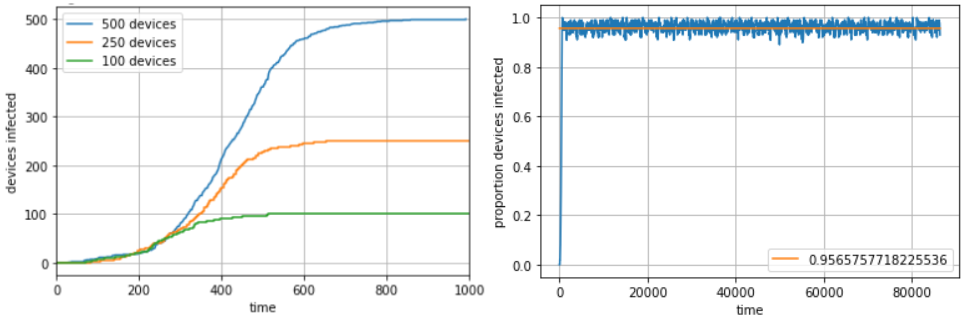
\includegraphics[width=\linewidth]{Figures/Compare_Device_Types.PNG}
    \caption{Botnet Growth for Always-Connected Devices (left) and Reboot-Capable Devices (right)}
    \label{fig:compare_device_types}
\end{figure}
\par

% ===================================== Compare Device Types ======================================
Figure~\ref{fig:compare_device_types} shows the typical behavior of both types of devices. \AC devices maintain their compromised state once infected, producing the expected classical logistic malware growth curve~\cite{stallings_brown_2015}. Once all devices have been infected, no new behavior can occur, so this device type is simulated for a shorter time. \RC devices, on the other hand, can remove their infection through rebooting as this wipes the in-memory malware on the device~\cite{Antonakakis2017_USENIX_Mirai_First_Study}. This produces a graph with a similar logistic growth at the beginning, which eventually settles into a steady-state as devices begin to reboot. This steady-state value is captured for most of the experiments conducted, as this provides an indication of how successful a specific frequency of rebooting is in preventing the botmaster to maintain a certain percentage of devices under their control.
\par
Simulation time is measured relative to the round trip time (RTT) parameter. In Figure~\ref{fig:compare_device_types}, the RTT is one second, so when the \AC devices are all infected within 1000 time units, this is equivalent to 1000 seconds, or 16.67 minutes. The simulation for \RC devices runs for 86400 time units, which for an RTT of one second, is equivalent to one day.

% =====================================  Reboot Frequency ======================================
\subsection{Impact of Rebooting on Percentage of Infected Devices}
\label{sub:rebooting_results}
Table~\ref{table:rebooting} presents the average percentage of infected devices for two networks of 100 devices with different RTTs. Uptime is calculated as the percentage of time a device is connected to the network. For example, a ten minute reboot period means that each device will reboot ten minutes after being connected, and with a fixed reboot length of one minute, has a 90.91\% uptime compared to the total eleven minutes of simulated time. The results indicate that as rebooting is performed more frequently, the average percentage of infected devices decreases, and bots on a slower network are impacted more severely by increased levels of rebooting. 

% old version
%Table~\ref{table:rebooting} presents the average percentage of infected devices for a network of 100 devices. Uptime is calculated as the percentage of time a device is connected to the network based on a one-minute reboot duration. For example, a ten minute reboot period means that each device will reboot ten minutes after being connected, and as the rebooting takes one minute, the uptime is 90\% compared to every ten minutes of simulated time. Botnet sizes are reported identical networks with two different latencies, so we can observe how network speed affects botnet propagation. \todo{3}{What do we see in the table?}

\renewcommand{\arraystretch}{1.5}
\begin{table}[h]
    \caption{\label{table:rebooting}Average percentage of infected devices for different reboot periods}
    \begin{tabularx}{\linewidth}{| c c >{\centering}m{0.263\linewidth} c |}
       \hline 
    	Reboot Period & Uptime & Average percentage  of devices infected (100ms RTT) & \multicolumn{1}{>{\centering}m{0.26\linewidth}|}{Average percentage of devices infected (1s RTT)}\\
    	\hline 
    	24hr & 99.93\% & 99.9\% & 99.0\%\\
    	1hr & 98.36\% & 97.8\% & 95.6\%\\
    	30min & 96.77\% & 96.0\% & 92.1\%\\
    	10min & 90.91\% & 89.6\% & 76.3\%\\
    	5min & 83.33\% & 80.7\% & 46.9\%\\
    	\hline
    \end{tabularx}
    %\vspace{-0.5cm}
\end{table}
\renewcommand{\arraystretch}{1}

% =====================================  Stealthy vs Active ======================================
\subsection{Stealthy vs Active Botnets}
\label{sub:stealthing_results}
%It may be advantageous for a bot to strike a balance between the percentage of time it spends propagating malware, and the percentage of time it stays idle.~\emph{Active} botnets such as Mirai~\cite{kolias2017_Mirai_DDoS} spend more time propagating themselves, so they can grow faster but risk being detected more easily, while \emph{stealthy} botnets will grow slower but are harder to detect. Table~\ref{table:stealthing} reports how different levels of activity, reboot period, and network speed impact the size of a botnet. In extreme cases where a stealthy botnet is operating on a network with a large RTT and frequent rebooting, the botnet is effectively prevented from spreading across the network. More generally, botnets with lower levels of activity achieve lower levels of infection, but a botnet can achieve high levels of stealth before its ability to propagate is affected. As with rebooting, an increase in RTT results in a more dramatic change in botnet size as activity level changes.

It may be advantageous for a bot to strike a balance between the percentage of time it spends propagating malware, and the percentage of time it stays idle.~\emph{Active} botnets such as Mirai~\cite{kolias2017_Mirai_DDoS} spend more time propagating themselves, so they can grow faster but risk being detected more easily, while \emph{stealthy} botnets will grow slower but are harder to detect. Table~\ref{table:stealthing} reports how different levels of activity, reboot period, and network speed impact the size of a botnet. Generally, botnets with lower levels of activity are shown to achieve lower levels of infection, however, bots can be very stealthy without losing much of their propagation capability. As with rebooting, an increase in RTT results in a more dramatic change in the percentage of infected devices as the activity level changes.

%Bots can also be very stealthy without losing much of their propagation capability, especially when devices are rebooted less frequently, as seen from the values reported in Table~\ref{table:stealthing}.

% old version:
%It may be advantageous for a bot to strike a balance between the percentage of time it spends propagating malware and the percentage of time it stays idle. Botnets that spend more time propagating themselves (\emph{active} botnets) can grow faster but risk being detected more easily, whereas botnets which spend more time idle (\emph{stealthy} botnets) will grow slower but are also harder to detect. While the Mirai malware typically is not concerned with hiding its presence~\cite{kolias2017_Mirai_DDoS}, it may be useful to see how different levels of activity affect its growth. Table~\ref{table:stealthing} describes how the activity level for a botnet impact its growth when paired with rebooting and varying network speeds.

\renewcommand{\arraystretch}{1.5}
\begin{table}[h]
    \caption{\label{table:stealthing}Average percentage of infected devices for different levels of botnet stealth}
    \begin{tabularx}{\linewidth}{| >{\centering}m{0.167\linewidth} c c  c |}
       \hline 
    	Percentage of time propagating malware & \multicolumn{1}{>{\centering}m{0.16\linewidth}}{Reboot Period} & \multicolumn{1}{>{\centering}m{0.24\linewidth}}{Average percentage  of devices infected (100ms RTT)} & \multicolumn{1}{>{\centering}m{0.24\linewidth}|}{Average percentage  of devices infected (1s RTT)}\\
    	\hline 
    	100\% & 1hr & 97.8\% & 95.6\% \\ 
    	50\% & 1hr & 97.7\% & 93.2\% \\
    	10\% & 1hr & 95.8\% & 69.6\% \\
    	1\% & 1hr & 71.5\% & 0.0067\% \\
    	100\% & 24hr & 99.9\% & 99.0\% \\
    	50\% & 24hr & 99.7\% & 98.7\% \\
    	10\% & 24hr & 99.4\% & 97.8\% \\
    	1\% & 24hr & 97.4\% & 86.0\% \\
    	\hline
    \end{tabularx}
    \vspace{-0.5cm}
\end{table}
\renewcommand{\arraystretch}{1}
% End Section

\section{Discussion}
\fontsize{10pt}{12pt}\selectfont
\label{sec:discussion}
% Begin Section
% Not needed: This section discusses the experimental results and their implications for the design of IoT networks.

% =====================================  Reboot Frequency ======================================
% \subsection{Impact of Rebooting on Botnet Size}
% \label{sub:rebooting_impact}

We can see from Table~\ref{table:rebooting} that for the more realistic network RTT of 100ms, the botnet size consistently remains very high even with frequent rebooting. This is a major problem for the high availability requirement of IoT networks, as even with network devices offline about 17\% of the time, the botnet is still able to infect above 80\% of devices. This frequency of rebooting is likely already undesirable for many IoT applications, with more frequent rebooting only further degrading the functionality of the uninfected devices. It is, therefore, evident that rebooting on its own is not effective as a primary defense against botnets; something more preventative such as blocking ports or changing default credentials would likely be much more effective.

% =====================================  Stealthy vs Active ======================================
% \subsection{Stealthy vs Active Botnet Size}
% \label{sub:stealthing_impact}
\par
The fact that a botnet can effectively hide its malicious presence on a network by simply remaining idle yet still commanding a large number of bots to perform an attack anytime is extremely concerning. In our experiments, where a botnet remains idle 99\% of the time on a network with one second RTT and hourly rebooting, the botnet cannot effectively spread, showing that stealthy botnets can be thwarted with these basic defenses. However, the level of botnet activity is outside the control of the IoT network designer, and without pertinent information, should not be expected to be low.

% =====================================  Network Speed ======================================
% \subsection{Impact of Network Speed on Botnet Size}
% \label{sub:network_speed_impact}
Both Table~\ref{table:rebooting} and Table~\ref{table:stealthing} show how network speed affects the growth of a botnet in various scenarios. In Table~\ref{table:rebooting}, the slower one second RTT network with very frequent rebooting is able to slow the botnet growth to an average size that may not be enough to perform an effective attack, while the slower network in Table~\ref{table:stealthing} is able to completely stop the stealthiest botnet in its tracks. It may be possible for a network designer to throttle their network to curb botnet spread, but this will impede the IoT network capability bringing us back to the security vs. performance issue. A network with one second RTT will likely not provide the level of service necessary for the IoT devices to perform as intended and thus cannot be considered a suitable defense against botnets.

% old version
%Both Table~\ref{table:rebooting} and Table~\ref{table:stealthing} show how network speed affects the growth of a botnet in various scenarios. A sufficiently slow network is shown in Table~\ref{table:rebooting} to lower the botnet size to a less severe value that may not be enough to perform an effective attack, while Table~\ref{table:stealthing} shows that a slow enough network can stop a stealthy botnet in its tracks. It may be possible for a network designer to throttle their network to curb botnet spread, but this will impede the IoT network capability bringing us back to the security vs. performance issue. A network with one second RTT will likely not provide the level of service necessary for the IoT devices to perform as intended and thus cannot be considered a suitable defense against botnets.
\par
%\mynote{3}{What about other experiments performed?}


Networks with different distributions of \AC and \RC devices did not produce significantly different results. Battery-operated devices were also considered, but these typically have lifespans too long to simulate with our current limitations.
% End Section

\section{Challenges Faced}
\fontsize{10pt}{12pt}\selectfont
\label{sec:challenges}
% Begin Section
The challenges encountered during the project come from two sources: technological limitations, and a lack of available studies on IoT device execution and rebooting times.~\par

At the time of writing, UPPAAL is available only as a 32-bit program on devices running Windows, which were the only device types available to us. This, coupled with UPPAAL's single-threaded simulations, led to a software bottleneck that ultimately limited what was feasible to simulate on our devices. UPPAAL also stores numbers as 16-bit signed integers, which became problematic as we were simulating many small interactions over a long time. It was necessary to include additional variables for the number of integer overflows, which allowed us to model a higher maximum value, but made recording values and specifying parameters more complicated.
\par
%The two factors that affect device execution timings and network latency, are both difficult to estimate. The default passwords used by Mirai have been mapped to the devices and vendors~\cite{Antonakakis2017_USENIX_Mirai_First_Study}, so we considered using this with knowledge of those vendors' devices to reason about execution times. In the end, we determined that this is likely negligible compared to latency as the propagation process is computationally simple and latency can vary wildly for different networks, so we selected a conservative time of 100 ms for most simulations.

The overall timing of the propagation process is determined by device execution times and network latency, which are both difficult to estimate. The default passwords used by Mirai have been mapped to the devices and vendors~\cite{Antonakakis2017_USENIX_Mirai_First_Study}, so we considered using this with knowledge of those vendors' devices to reason about execution times. In the end, we determined that this is likely negligible compared to latency as the propagation process is computationally simple. Latency can vary wildly for different networks, so we selected a conservative time of 100 ms for most simulations.

\par
Reboot frequency and the duration of a device's reboot process were also difficult to determine. We explored works on rebooting times, user behaviors, and manufacturer recommendations for reboot frequency, but were mostly unsuccessful. A few IoT device manuals~\cite{comtrend_2012} suggest that their reboot process takes about 60 seconds, so we decided to use this time in our model. As we were unable to find any concrete information on the recommended reboot frequency, we adjusted our research focus to see how varying this affects the botnet size.
\par
We should note that UPPAAL is a research tool and is under active development, so many of the technical challenges may be solved in future versions of the tool. Access to faster computation resources and alternative operating systems would allow for a wider range of scenarios to be tested on our model. The model is designed to allow timings to be altered easily, so if papers are published in the future on IoT rebooting behaviors, the model can be updated accordingly to obtain potentially more accurate results.
% End Section

\section{Related Work}
\fontsize{10pt}{12pt}\selectfont
\label{sec:literature_review}
% Begin Section
% %====================================
% \subsection{Studies on the Botnet Infection Process}
% \label{sub:studies_botnet_infection_process}
The Mirai botnet has been studied in great detail in \cite{kolias2017_Mirai_DDoS, kambourakis2017mirai, Antonakakis2017_USENIX_Mirai_First_Study}, forming the basis of our developed model.~\cite{kolias2017_Mirai_DDoS} and~\cite{Antonakakis2017_USENIX_Mirai_First_Study} describe the roles of bots and each component of the botnet infrastructure, while~\cite{kambourakis2017mirai} gives an in-depth description of the specific activities each infected bot performs in propagating the malware. The information gained from these three studies allowed us to accurately depict each component of the botnet infrastructure and their interactions to observe and examine the botnet behavior.

%====================================
% \subsection{Modelling Attempts}
% \label{sub:other_botnet_models}
The general infection process of botnets has been modeled using various other modeling formalisms.~\cite{tanaka2017modeling} and~\cite{tanaka2019_PN_Botnet} use agent-oriented Petri nets to model the Mirai and Hajime botnets, exploring the possibility of using rebooting and Hajime as an innocuous botnet to reduce the Mirai infection rate. Both botnets are, however, modeled only as black box entities without modeling the underlying infrastructure, and the scalability of such an approach is limited as the authors fail to extend the network beyond 25 nodes. Epidemiological approaches, such as~\cite{kephart1993epidemiological} and~\cite{jerkins2018epidemiological}, effectively model time, but are limited in the amount of detail that can be modeled. Other attempts involve the use of game theory, machine learning, and economic models~\cite{wainwright2019_Botnet_Models}. Our approach aims to combine the benefits, in particular, of Petri Nets and Epidemiological models, by providing considerations for time and concurrency while also presenting an extensible model with a fine-grained level of adjustable detail.
\par
%====================================

%====================================
% \subsection{Other Methods of Study}
% \label{sub:other_methods_of_study}
Other approaches to study botnets involve collecting data from real-world network traffic and devices, including the use of honeypots~\cite{Antonakakis2017_USENIX_Mirai_First_Study, silva2013_Botnet_Survey}, DNS traffic logs~\cite{Antonakakis2017_USENIX_Mirai_First_Study, feily2009botnet_detection}, tracing DDoS attacks back to their source~\cite{Antonakakis2017_USENIX_Mirai_First_Study}, and scanning for devices with bot-like behavior~\cite{Antonakakis2017_USENIX_Mirai_First_Study, feily2009botnet_detection, herwig2019hajime, acarali2016http_botnets}. These methods have the benefit of generating real-world data, which can lead to potentially more accurate results. However, the data collection process requires time and violates ethical considerations, making those approaches out of scope for this project.
%====================================
% End Section

\section{Conclusion}
\fontsize{10pt}{12pt}\selectfont
\label{sec:conclusion}
% Begin Section
% ================================= What did we gain through this?  ===================================
% In this project, we designed and implemented a model of the Mirai botnet using timed automata in UPPAAL in order to observe how botnet growth is impacted in various scenarios. Device rebooting is shown to be ineffective at reducing the spread of the botnet unless performed at levels which would degrade the functionality of the IoT device network. Both decreased network speed and level of botnet activity are shown to make a botnet more susceptible to this use of rebooting as a defense.
% \par
% While our hardware and operating system constraints put some limit on the complexity we were able to study, the existing model is highly scalable. Access to more powerful hardware and an alternative operating system such as Linux would allow larger and faster networks to be studied with the same level of accuracy.

%\mynote{2}{\underline{COPIED FROM INTRO:} The knowledge gained through this study will allow one to reinforce their understanding of the botnet infection process as well as identify areas of limited understanding. Additionally, they will gain insight into the effectiveness and viability of rebooting and weigh it against other available defensive measures to provide suitable recommendations.}

In this project, we developed a timed automata model of the Mirai botnet in UPPAAL and observed the infection rate and interactions between individual botnet entities. Additionally, we considered clusters of different device types and simulated large networks of such clusters to see the influence of different device distributions. Finally, we examined the impact of rebooting on both stealthy and active botnets to determine the frequency of rebooting capable of curbing the botnet growth.
\par
Our analysis shows that device rebooting, by itself, is ineffective at reducing the spread of botnets unless performed at a level that would degrade the performance of a device or the availability of the IoT network. The level of botnet activity, as well as decreased network speed, are shown to be notable factors that affect the maintainability of a large botnet over an extended period. While the breadth of our analysis was limited by the available hardware, the existing model is highly scalable and allows for easy adjustment of parameters to simulate myriads of scenarios.
\par
In future work, we aim to explore the effectiveness and viability of other suggested solutions in a network consisting of over ten thousand devices. In particular, we wish to see the impact of patching as well as how the inclusion of devices with limited battery lifespan affect our analysis.


% End Section
% ==================================================================================================




% ==========================================REFERENCES==============================================
\fontsize{10pt}{12pt}\selectfont
\bibliographystyle{ieeetr}
\bibliography{citations}
% ==================================================================================================


\end{document}
